\chapter{Environment modeling}

\section{Overview}
\label{chap:env_overview}

The environment is coded as a constant base upon which we build the entire project. This choice has been derived from two main reasons. \textit{The first one} is that the environment's nature doesn't change in each different step, thus it behaves always in the same way. \textit{The second one} is to better compare the results of different situations without introducing a bias in the inputs we feed the algorithm.

In order to better simulate a real case scenario and to maintain consistency between the different learners, the environment contains all the required functions and data needed by the simulator to compute the outcome of every day given the initial parameters. Each day, the simulator asks for a \textit{budget assigment} and returns the obtained rewards to the learner, which, after adjusting its parameters to maximize the reward for the next predictions, will be ready for the next day.

What will change between steps is how much data the learner will be given as input by the simulator; as a matter of fact, from the learners' perspective, the environment is \textit{"masked"} and it will contain only the known data for each step (different for each point of the project).

\section{Hypotheses}
\label{sec:env_hypoteses}

In this section the specific assumptions related to the environment modelling are listed.

\begin{itemize}
    \item Each consumer is characterized by 2 binary features, for instance: occupation (student/worker) and gender (female/male). These features will define the 3 different user classes that we want to target in our advertisement campaign.
    \item The probability for each class to be able to enter the website is fixed and unknown from the learner's perspective. It can be seen as a percentage over the population that we are focusing with our ads.
    \item Each user class is distinguishable by an $\alpha_i$ function expressing the ratio of users landing on the web-page where product $P_i$ is shown as the primary one. More clearly, given a campaign every class is characterized by a different profile of $\alpha$ functions.
    \item The competitor's budget is considered to be constant assuming a \textit{non-strategic player}.
\end{itemize}

\section{Model Choice}
\label{sec:env_Motivation}

We chose to model the $\alpha$ functions as \textit{exponential} functions identified by an \textit{reservation price}, an \textit{upper bound} and a \textit{maximum useful budget}. In particular their \textit{upper bound} represents the maximum expected number of interactions possible and the \textit{maximum useful budget} is the amount of budget after which any budget increase would not lead to a ratio increase, meanwhile the \textit{reservation price} is defined as the maximum price at which the user will buy a given product.

Moreover, having three different parameters to tune gives us the possibility to better differentiate each user class.

\section{Code Analysis}
\label{sec:env_Code Analysis}

\subsection{Environment}
The environment is composed by different objects and functions which model the users' interactions on the web-page, how users react given different budgets and how the final reward is obtained from a day of interactions.

\begin{enumerate}
    \item Environment Data

    These two data classes contain all the relevant information for the environment. Most of the parameters for the Environmnet Data class are completed by default at creation time, however, each one of them can be specified when the class is constructed to create a custom environment. Notably, the Environmnet Data class can be passed to the function \textit{get\_day\_of\_interactions} which generates a whole day of interactions from the specified environment.

    \begin{lstlisting}[style=Python]
\@@dataclass@@/
class EnvironmentData:

    """Dataclass containing environment values. Should be constructed passing
    the rng parameter, which is the only one not defined by default. The other
    parameters are set up correctly by the dataclass constructor, with default
    values as shown below. Setups correctly everything about the environment.
    After constructing this class, it can be passed to the function
    get_day_of_interactions. To construct it with different values they can
    simply be specified when the class is constructed.
    """

    # The total budget to subdivide
    total_budget: int

    # Probability of every class to show up. They must add up to 1
    class_ratios: List[float]

    # Features associated to every class
    class_features: Dict[Tuple[Feature, Feature], int]

    # Price of the 5 products
    product_prices: List[float]

    # List of class parameters for each class and product, implemented as list
    # of lists of UserClassParameters. Each class has distinct parameters for
    # every product
    classes_parameters: List[List[UserClassParameters]]

    # Lambda parameter, which is the probability of osserving the next secondary
    # product according to the project's assignment
    lam: float

    # Max number of items a customer can buy of a certain product. The number of
    # bought items is determined randomly with max_items as upper bound
    max_items: int

    # Products graph's matrix. It's a empty matrix, should be initialized
    # with populate_graphs
    graph: np.ndarray

    # List that constains for every i+1 product the secondary i+1 products
    # that will be shown in the first and second slot
    next_products: List[Tuple[int, int]]

    # Controls the randomness of the environment
    random_noise: float
    \end{lstlisting}

    \item Masked environment

    In addition, the Masked Environment Data class is a parallel data class w.r.t. Environment Data with the purpose of \textit{hiding crucial information} to the learners since each type of learner should only have access to a subset of all the information available in the environment dictated by the type of learner.

    The masked environment isn't strictly needed in the project since the learners could easily ignore the extra information, however, we wanted to face the problem with an approach aimed towards reusability and extendability and in this case (as in many others down the line) we opted for a more \textbf{generalizable} solution.

    \item Modelling user interactions

    With the aid of the functions \textit{simulate\_interaction} and \textit{generate\_interactions} we can compute a single set of interactions starting from a page, returning a set of intermediate results called \texttt{blueprints} which can be used to generate actual interactions following the user behavior defined in section \hyperref[sec:intro_overview]{Overview}.

    \item Overall result of a day

    The \textit{get\_day\_of\_interactions} function is the able to generate a whole day of interactions utilizing the aforementioned functions and accepting a budget parameter obtained by the learner through the simulation and used to influence the distribution of users on different pages; it also needs the \textit{Environment Data} and the total population of visitors of the e-commerce website for that day.
\end{enumerate}

It is worth to note that the Environment isn't necessarily deterministic, in fact, for the sake of representing a real scenario, most of the values that are not known a priori are \textit{randomly generated} and every variable that evolves through time without our direct control has elements of randomness to it (for instance, each day we randomly get the number of active total users in our scenario by using a gaussian distribution with tunable mean and standard deviation).

Even though most of the randomness is tunable and controlled through seeded generators, there are still \textbf{impactful elements of non determinism} (i.e. the Dirichlet distribution) that are not possible to control in any way.

\subsection{Simulation}

The \textbf{Simulation} class is the main engine that brings together \textit{learners} and \textit{environment} by making them interact with each other while offering an interface to customize the execution. It mainly uses functions already definded in the environment to compute the rewards and to adjust the parameters as the learner improves.

The basic idea of the simulation is to simulate a real scenario day by day using the environment to generate interactions with the website according to the budgets that the current learner proposed and then, feed the results back to the learner to make it actually learn.

Repeating the simulation execution step for each day until an arbitrary \textbf{time horizon} is reached grants us all the data needed to evaluate the performance of our learner.

The main method of interaction with a simulation is the \texttt{simulate} function, which runs the simulation for a specified number of days, this preserves the status of the simulation, enabling consecutive calls of this function in order to simulate multiple batches of days step-by-step.
Inside the simulation module exist some quality-of-life functions such as \texttt{create\_n} and \texttt{simulate\_n}, which respectively create and call simulate on batches of $n$ simulations; this is useful to collect average results over a large number of runs.

\begin{lstlisting}[style = Python]
def create_n(
    rng: Generator,
    env: EnvironmentData,
    step: Step = Step.ZERO,
    n: int = 2,
    n_budget_steps: int = 20,
    population_mean: int = 100,
    population_variance: int = 10,
    **learner_params,
):

    """Helper function that simplifies the creation of multiple equal simulations
	at once
    Arguments:
        n: number of simulations to create
        rng: randomness generator
        env: environment where the simulation is going to be run
        step: step number of the simulation, related to the various steps requested
        by the project specification and corresponding to which properties
        of the environment are masked to the learner and to which learner is going
        to be instantiatiated
        n_budget_steps: number of steps in which the budget must be divided
        population_mean: expected value of the number of new potential
        customers every day
        population_variance: variance of the daily number of potential customers
        learner_params: various parameters used to created the selected learner
    Returns:
        A list of new simulations with the parameters specified
    """

    return [
        Simulation(
            rng,
            env,
            step=step,
            n_budget_steps=n_budget_steps,
            population_mean=population_mean,
            population_variance=population_variance,
            **learner_params,
        )
        for i in range(n)
    ]

def simulate_n(
    simulations: List[Simulation],
    n_days: int = 100,
    show_progress_graphs: bool = False,
):

    """Helper function that simplifies the act of running multiple simulations with
	the purpose of visualization of the results
    Arguments:
        simulations: list of simulation objects that will be run
        n_days: number of days to run each simulation for
        show_progress_graphs: if set to True, will visualize the learner progress graphs
        (if implemented) at each iteration
    Returns:
        A list containing all the collected rewards obtained by running all
		the simulations.
    """

    rewards = []

    for sim in simulations:
        sim.simulate(n_days, show_progress_graphs)
        rewards.append(sim.rewards)

    return rewards
\end{lstlisting}

\subsection{Simulation example}

Example of two simulation runs for learners in an environment with total\_budget = 400 and population\_mean = 1000.

\begin{center}
    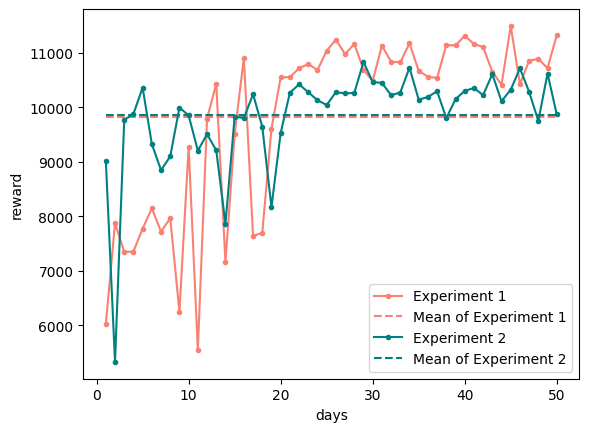
\includegraphics[scale=0.5]{img/Graphs/env_sim/image1.png}
\end{center}
